\chapter{Event Simulation and Data Samples}\label{ch:EventGenSim}

Analysis of data collected by experiments requires the knowledge of how various particles (also referred to as physics objects at various occasions 
in this thesis) behave in the detector, which can be foreseen by simulating the events. Even before the experiment begins, the simulation chain 
provides valuable inputs for the very design of the experiment, along with its various sub-detectors, and guides the reach for most interesting physics 
program in pursuit of new physics. Predicting the results of \pp collisions involves the modelling of several aspects, such as the structure of the 
proton, the scattering cross section, the decay of unstable particles, and the hadronization of quarks and gluons into jets. 
These algorithms are based on random numbers weighted by the probability of the underlying processes occurring in particle collisions and are 
referred to as ``event generation''. Event generation forms the first step in the simulation chain.
%These modeling produce randomly hypothetical events with kinematic and topological distributions predicted by the theory and referred to as ``event 
%generation'', which forms the first step in the simulation process. 
There are several event generators or Monte Carlo (MC) generators~\cite{Buckley:2011ms,Dobbs:2004qw} as they are often called, available for a wide 
range of collider experiments, such as \pythia~\cite{Sjostrand:2006za}, \madgraph~\cite{Alwall:2014hca}, and \herwigpp~\cite{Bahr:2008pv} to name a few.
%Several event generators or Monte Carlo (MC) generators~\cite{Buckley:2011ms,Dobbs:2004qw} have been developed by different group of physicists for 
%a wide range of collider experiments and each concentrates on different purposes and has therefore different pros and cons for a particular task. 
The details of implementation of the underlying physics processes are different in each of these generators, but the fundamental idea of simulating
events to match the real collision scenario remains the same. 

After generation of events, the response of the detector to physics objects must be modelled. The generated events are passed through detector 
simulation to obtain the effect of material on various particles. The information for the input event received after detector simulation are used 
for the reconstruction of various physics objects and are analyzed using the program used for analyzing experimental data. The simulation data 
along with the experimental data are important for estimating efficiencies, expected backgrounds, determining uncertainties, and adjusting the 
trigger parameters. The simulation and experiment are, thus, interleaved through an iterative loop and the interpretation of the experimental data 
depends, to some degree, on the assumptions made in the simulation tools. 

This chapter describes the methods and tools used for simulating \pp collision events in the CMS detector. A description of the
MC generators and event simulation used to model the signal process $\pp\rightarrow\qstar\rightarrow\gamjet$, and potential physics backgrounds
has been given.

\begin{figure}[h!]
\centering
%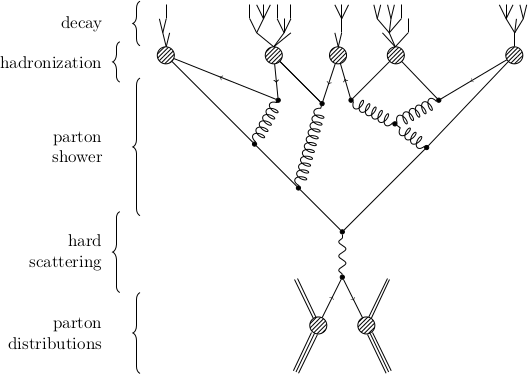
\includegraphics[width=14cm,height=10cm]{ch3/figures/EventGeneration_1.png}
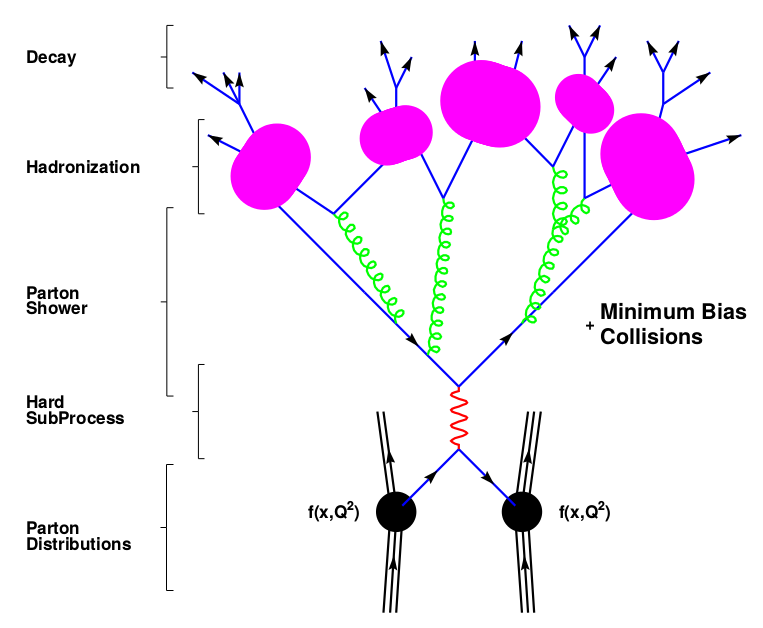
\includegraphics[width=14cm,height=12cm]{ch3/figures/EventGeneration.png}
\caption{Illustration of a generated event depicting incoming partons undergoing interaction via a hard scattering process, and outgoing partons
showering and hadronizing.}
\label{fig:EventGeneration}
\end{figure}

\section{Event Generation}
Event generation forms the first step in the simulation process and is usually performed in various steps following a modular approach.
\subsection{Hard Scattering and QCD Radiation}
The simulation starts with partons from the colliding protons interacting via hard scattering as shown in \fig{\ref{fig:EventGeneration}} from 
Ref~\cite{Dobbs:2004qw}, producing SM particles such as quarks, leptons, photons, or some new hypothetical particle (say \emph{preon})~\cite{Pati:1975md,Eichten:1983hw,Baur:1987ga} as predicted by new physics models. The cross section and the differential kinematic distribution 
for a $2\to2$ sub-process in hadronic collisions at tree level are calculated as follows:
%\begin{multline}
\begin{equation}
\sigma(ab\rightarrow{cd})=\sum_{ab}\int_{0}^{1}\int_{0}^{1} f_{a}(x_{1},\mu_{F}^{2})f_{b}(x_{2},\mu_{F}^{2})\hat{\sigma}_{ab\rightarrow{cd}}
                           \left(\hat{s},\alpha_{s}(\mu_{R}^{2}),\frac{Q^{2}}{\mu_{F}^{2}},\frac{Q^{2}}{\mu_{R}^{2}}\right)dx_{1}dx_{2} 
% \\ + f_{q}^{p}(x_{1},Q^{2})f_{\bar{q}}^{p}(x_{2},Q^{2})\hat{\sigma}(q\bar{q}\rightarrow{g\gamma})\Big] dx_{1}dx_{2} 
\label{eq:gamJetXS}
\end{equation}
%\end{multline}
where $\hat{s}$ is given by the relation $\hat{s}=x_{1}x_{2}s$, with $s$ being center-of-mass energy of the collider, $Q$ is the characteristic hard 
scale of the interaction, $\mu_{F}$ is the factorization scale, and $\mu_{R}$ is the renormalization scale. Both the $\mu_{R,F}$ scales are arbitrary 
parameters of a fixed order calculation. At all orders of the pertubative expansion, the cross section must be independent of them (i.e. $\partial
\sigma/\partial\mu_{R} = \partial\sigma/\partial\mu_{F} = 0$). For all practical calculations of cross sections at a fixed order, it is assumed that 
$\mu_{R}=\mu_{F}=Q$. The function $f_{a}(x_{1},\mu^{2}_{F})$ represents the probability density for finding a parton $f_{a}$ in the proton, also 
referred to as the Parton Distribution Function (PDF), carrying a fraction $x_{1}$ of the initial proton momentum when the factorization scale is 
$\mu^{2}$. There is also a possibility for parton $f_{a}$ to carry momentum fraction $x_{2}$ and parton $f_{b}$ to carry $x_{1}$.
The $\hat{\sigma}_{ab\rightarrow{cd}}$ represents the parton level cross section for the hard 
process leading to $cd$ final state from the initial partons $a$ and $b$. The fully differential parton level cross section is calculated as the 
product of the corresponding matrix element squared, averaged over inital state spin and color degrees of freedom, sum over the spins of the final
state particles, and the parton flux. The cross section is computed using \eqn{\ref{eq:gamJetXS}} with MC integration techniques and considering 
uniformly distributed random numbers for variables, $\theta$, $\phi$, $x_{1}$, and $x_{2}$.

Our understanding of the QCD is incomplete in the sense that a derivation from first principles of parton distributions does not yet exist, although 
some efforts are being made in lattice QCD studies. It is, thus, necessary to rely on parameterizations, where experimental data are used along with 
evolution equations~\cite{Altarelli:1977zs} for the $Q^{2}$ and $x$ dependence. The PDFs are determined by global fits to data from 
deep inelastic scattering, Drell-Yan processes, and jet production at high energies. The PDFs used in the analysis described in this 
thesis is from the Coordinated Theoretical Experimental Project on QCD (CTEQ) group~\cite{Nadolsky:2008zw}. In particular, the parametrization, 
CTEQ6L1~\cite{Pumplin:2002vw,Martin:2009iq}, which provides an accurate description to the collision data, has been used. 
%The PDFs are fed into parton \emph{evolution} equations, which are models of perturbative QCD (pQCD). These extrapolate the Q$^{2}$ and $x$ dependence of the PDF.

\subsection{Parton Shower, Underlying Event and Hadronization}
In processes that contain charged and/or colored objects in the initial- and/or final-state, gluon and/or photon radiation may give a large correction
to the overall topology of the event. After a hard scattering event has been generated, higher order effects are added by using parton shower 
simulation, which allows partons to split in pairs of other partons (for example, $g\rightarrow{q\bar{q}},q\rightarrow{qg}$).
%After simulating a hard process, the final state is composed of quarks and gluons. Few MC generators starts with the leading order (LO) hard 
%sub-processes and higher order effects are added by evolving the event using parton shower simulation, that allows partons to split into pairs of 
%other partons (\ie, $g\rightarrow{q\bar{q}},q\rightarrow{qg}$). While others include next-to-leading-order (NLO) pQCD diagrams leading to three or 
%more partons in the final state before starting the parton showering process.
The resulting partons may branch further, leading to a large number of quarks and gluons, which are grouped together into color singlet (or colorless) 
hadrons known as hadronization, in accordance with the quark confinement model. A schematic diagram depicting the entire process is shown in \fig{\ref{fig:EventGeneration}}. 
\begin{figure}[h!]
\centering
%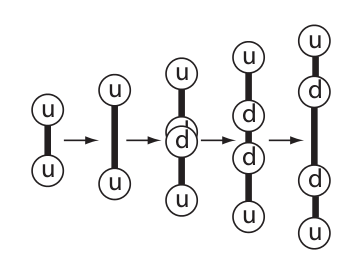
\includegraphics[width=7cm,height=5cm]{ch3/figures/LundModel.png}
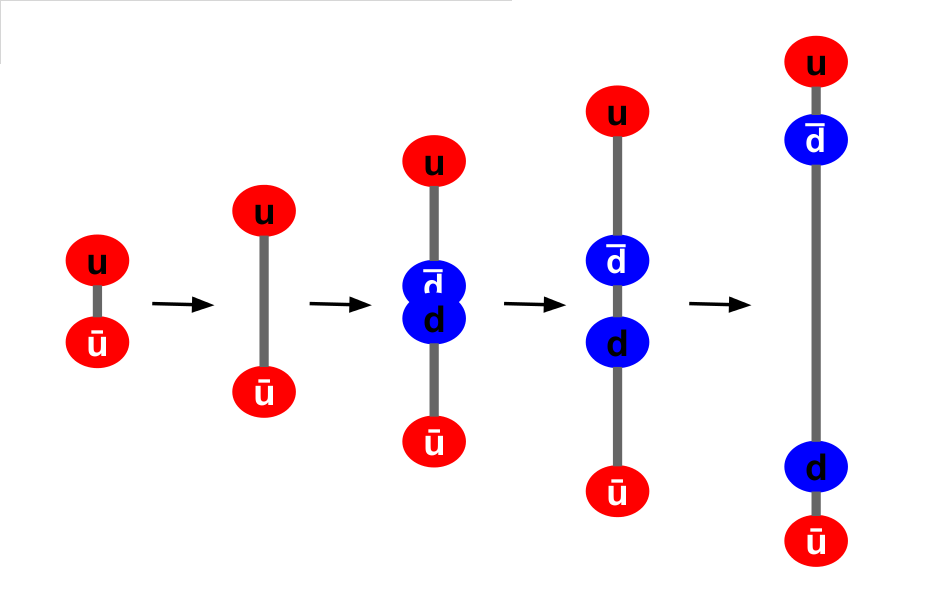
\includegraphics[width=9cm,height=6.5cm]{ch3/figures/Lund_String_Model.png}
\caption{Hadronization of an initial state of two quarks where another quark pair is created from the energy stored in the color field.}
\label{fig:LundModel}
\end{figure}

Pertubative QCD, formulated in terms of quarks and gluons, is valid only at short distances. At long distances, QCD becomes strongly interacting and 
perturbation theory can not be applied. Hadronization process takes place over relatively larger distances (low momentum exchange) when compared to 
the hard scattering, so it cannot be modeled by pQCD. 
%In addition, the hadronization process involves scattering with low momentum exchange. 
A common model used for this is the Lund String Model~\cite{Sjostrand:1986hx}, which is briefly described below. 

Lund String model is based on probabilistic and iterative approach. It starts with color field as a one-dimensional `string' between two colored 
quarks as illustrated in \fig{\ref{fig:LundModel}}. As the partons ($u$ and $\bar{u}$) move apart from their common production vertex, the string
 is stretched between the $u$ and the $\bar{u}$. The transverse dimensions of the string are of the order of the hadronic size ($\approx 1\unit{fm}$)
and are assumed to be uniform along its length. From hadron spectroscopy, the amount of energy per unit length (also sometimes referred to as 
the string constant) of the string is inferred to be $\kappa\approx1\unit{GeV/fm}$. As the $u$ and $\bar{u}$ move apart, the potential energy of 
the string increases, and the string may break by creating a new $q\bar{q}$ (say, $d\bar{d}$) pair, so that we have two color singlet systems 
$u\bar{d}$ and $d\bar{u}$. The string break up process proceeds until only colorless hadrons remain and then, these themselves may decay into 
leptons or stable hadrons. The final system of particles emerges aligned roughly along the original $u\bar{u}-$axis.
%Lund String Model starts with color field as a one-dimensional `string' between two colored quarks as illustrated in \fig{\ref{fig:LundModel}}.
%Because of triple gluon coupling, color flux lines do not spread throughout the space (unlike electromagnetic fields), but are restricted to a
%narrow region. The amount of energy per unit length of the string is phenomenologically found to be $\kappa\approx1\unit{GeV/fm}$. A new pair
%of quarks can be created from the available energy in the field.  The original system of quarks breaks into smaller pieces iteratively,
%until only colorless hadrons remain, that may themselves decay into leptons or stable hadrons. The final system of particles emerge aligned
%along the original $q\bar{q}-$axis. 

One more important thing that needs to be modelled for generating a real collision-like event is the modelling of the underlying event. 
The partons left over in the proton after a parton is pulled out to participate in the hard scattering event is referred to as the Beam
remnant. They have small \pt  ($\sim1\unit{GeV}$), but are connected through color fields to the hard scattering. In MC generators such as
\pythia, these beam remnants are allowed to interact ( multi parton interaction), shower and decay themselves. The result of these beam 
remnant interactions is generally referred to as the ``underlying events''.

\subsection{Monte Carlo Event Generators}
As mentioned earlier, several MC event generators exist in the present day world. Many of these are general-purpose ones while others deal with 
specific processes. Some of the general-purpose generators include \pythia~\cite{Sjostrand:2006za}, \madgraph~\cite{Alwall:2014hca}, 
\herwigpp~\cite{Bahr:2008pv}, \alpgen~\cite{Mangano:2002ea}, and \sherpa~\cite{Gleisberg:2008ta}. The text in the following subsections 
briefly describes the details of some of the MC simulation programs used to model the signal and background processes for the search of excited quarks 
depending on the peculiarity of the respective final states.

\subsubsection{Pythia}
\pythia~\cite{Sjostrand:2006za} is one of the oldest and well established general purpose MC event generators used for lepton and hadron colliders. 
It uses the Lund string fragmentation model~\cite{Sjostrand:1986hx} to describe hadronization and consists of a library of about 240 different
hard scattering processes involving 2 incoming partons and 1 or 2 outgoing particle at the LO. It is able to simulate all the generation steps
explained earlier. Initial- and final-state showers are added to provide more realistic configurations. The signal samples ($\pp\rightarrow\qstar
\rightarrow\gamjet$), and SM backgrounds QCD \gamjet and dijet used in this analysis are generated using \pythia event generator and are described
in more detail in Chapter~5.

\subsubsection{Madgraph}
\pythia is an effective event generator for describing $2\rightarrow{2}$ process but most of the processes observed in experimental
collisions have additional hard particles in the final state. The \madgraph~\cite{Alwall:2014hca} matrix element generator allows
one to simulate amplitude for any process up to 9 particles in the final state. It automatically generates the amplitudes for relevant
sub-processes via the ALOHA package~\cite{deAquino:2011ub}. Events are passed as parton level files in the standard
event format known as Les Houches format (LHE files)\cite{Alwall:2006yp}. These LHE files are then passed to \pythia for the parton showering
and hadronization before passing them to detector simulations. The matching of matrix element (ME) to parton shower (PS) also happen
at this point and it is important to perform the merging to avoid double counting of emissions in overlapping phase space regions. Two methods
available to perform the merging are, CKKW algorithm~\cite{Krauss:2002up}, and MLM scheme~\cite{Mangano:2001xp}. 

The \madgraph samples used in this thesis contain LO calculations for \pp collisions leading to $W\gamma$, $W+$jets, and $Z\gamma$ in the final state. 
These backgrounds are discussed in more detail in Chapter~5.
%\subsubsection{TAUOLA}
%TAUOLA~\cite{Was:2000st} is a MC program used explicitly to model the decays of $\tau-$leptons with proper description of polarization. The
%package utilizes an individual phase space generator for each decay channel including specific modeling of the weak and hadronic current. It can
%also be interfaced to other event generators that produce the hard scattering process, \ie, \pythia and \madgraph.

\section{Detector Simulation}
The theoretical predictions form an integral part in the planning of the CMS experiment and help define the experimental strategies
and design of the detector including software needed for the operation. These predictions need to reproduce the interaction processes 
taking place in hadron collisions and the interaction of the emerging particles with the various detector systems as closely as possible.
After simulating hard scattering to final state particles, further simulation is performed on their interaction within the CMS
detector. The complexity of the detector requires very sophisticated programs to properly reproduce the detector behavior in the presence of 
particles from proton collisions. The detailed simulation is performed within the CMSSW~\cite{cmsTDR} framework using the 
\geant~\cite{Agostinelli:2002hh} toolkit. The \geant package relies on accurate description of all aspects of the detector including full geometry, 
material of the detecting devices and the dead material (\eg cables, support, cooling etc) to simulate the response to the interacting particle. The 
core of \geant is a set of physics models to handle the interactions of particles with material over a wide ranges of energy (from few hundreds of eVs 
to a few TeV). Taking particles from the event generator as input, it propagates them through the detector taking into account the magnetic field (for 
charged particles) and any interactions between the particle and material such as bremsstrahlung, multiple 
scattering and photon conversion. Then, the response of detector is built further by emulating the response of the readout
and trigger electronics of the detector to the simulated hits, through the process of digitization. Noise and other effects are also 
considered during this step. Finally, a raw output similar to that of the real data event format is obtained. All subsequent stages, 
such as event reconstruction as described in the next chapter, uses the same input collection and behave identically whether running on simulated 
events or real data.

\section{Simulated Samples}
The complete set of the signal and background MC samples used in this thesis are listed in \tab{\ref{Table:SigSamples}} and 
\tab{\ref{Table:BkgSamples}} respectively. All the MC samples were simulated and reconstructed using the CMSSW version 5\_3\_8\_patch1.

The \qstar signal MC were generated using \pythia6.426 with the underlying event tune Z2$^{\ast}$. This tune is described in more detail in 
Ref.~\cite{Chatrchyan:2011id,Field:2010bc}. To generate \qstar of $\mqstar=1\unit{TeV}$ and coupling, $\Lambda=1.0$ following set of parameters 
were used :
\begin{verbatim}
`MSEL        = 0     !User selected',
`MSTP(6)     = 1     ! excited quark',
`MSUB(147)   = 1     ! dg--> d*',
`MSUB(148)   = 1     ! ug--> u*',
`PMAS(343,1) = 1000. ! d* mass',
`PMAS(344,1) = 1000. ! u* mass',
`RTCM(41)    = 1000. ! Scale parameter Lambda',
`RTCM(43)    = 1.0   ! f=1   SM coupling',
`RTCM(44)    = 1.0   ! fprime=1  SM coupling',
`RTCM(45)    = 1.0   ! f_s=1 SM coupling',
`4000001:ALLOFF         !Turn off all u* decays',
`4000001:ONIFMATCH 1 22 !Turn on u*->u Photon',
`4000002:ALLOFF         !Turn off all d* decays',
`4000002:ONIFMATCH 2 22 !Turn on d*->d Photon',
\end{verbatim}
%---------------TABLE FOR MC samples-------------------
\begin{table}[h!]
\begin{center}
%\begin{ruledtabular} 
\resizebox{16cm}{!}{
%\begin{tabular}{|l|c|c|c|}
\begin{tabular}{lccc}
\hline
{\bf Signal Samples } & {\bf Events } & {\bf Cross section (pb)} & {\bf Couplings}\\
\hline
\hline
QstarToGJ\_M-700\_TuneZ2star\_8TeV-pythia6  & 60065 & 24.85 & 1.0 \\
QstarToGJ\_M-1000\_TuneZ2star\_8TeV-pythia6 & 60192 & 4.18 & 1.0 \\
QstarToGJ\_M-1200\_TuneZ2star\_8TeV-pythia6 & 60120 & 1.552 & 1.0 \\
QstarToGJ\_M-1500\_TuneZ2star\_8TeV-pythia6 & 60138 & 4.124$\times$10$^{-1}$ & 1.0 \\
QstarToGJ\_M-1700\_TuneZ2star\_8TeV-pythia6 & 60256 & 1.843 $\times$10$^{-1}$& 1.0 \\
QstarToGJ\_M-2000\_TuneZ2star\_8TeV-pythia6 & 120105 & 5.858 $\times$10$^{-2}$ & 1.0 \\
QstarToGJ\_M-2500\_TuneZ2star\_8TeV-pythia6 & 120127 & 9.768$\times$10$^{-3}$& 1.0 \\
QstarToGJ\_M-3000\_TuneZ2star\_8TeV-pythia6 & 120032 & 1.755$\times$10$^{-3}$& 1.0 \\
QstarToGJ\_M-3500\_TuneZ2star\_8TeV-pythia6 & 160095 & 3.241$\times$10$^{-4}$& 1.0 \\
QstarToGJ\_M-4000\_8TeV-pythia6 & 159703 & 6.045$\times$10$^{-5}$& 1.0 \\
QstarToGJ\_M-4500\_8TeV-pythia6 & 306561 & 1.170$\times$10$^{-5}$& 1.0 \\
\hline\hline
QstarToGJ\_M-700\_fhalf\_8TeV-pythia6 & 59013 & 6.249 & 0.5 \\
QstarToGJ\_M-1000\_fhalf\_TuneZ2star\_8TeV-pythia6 & 60196 & 1.064 & 0.5 \\
QstarToGJ\_M-1500\_fhalf\_TuneZ2star\_8TeV-pythia6 & 60053 & 1.05$\times$10$^{-1}$& 0.5 \\
QstarToGJ\_M-2000\_fhalf\_TuneZ2star\_8TeV-pythia6 & 120012 & 1.484$\times$10$^{-2}$& 0.5 \\
QstarToGJ\_M-2500\_fhalf\_TuneZ2star\_8TeV-pythia6 & 120054 & 2.425$\times$10$^{-3}$& 0.5 \\
QstarToGJ\_M-3000\_fhalf\_TuneZ2star\_8TeV-pythia6 & 120059 & 4.304$\times$10$^{-4}$& 0.5 \\
QstarToGJ\_M-3500\_fhalf\_TuneZ2star\_8TeV-pythia6 & 160008 & 7.586$\times$10$^{-5}$& 0.5 \\
QstarToGJ\_M-4000\_fhalf\_8TeV-pythia6 & 159808 & 1.258$\times$10$^{-5}$& 0.5 \\
QstarToGJ\_M-4500\_fhalf\_8TeV-pythia6 & 160000 & 1.929$\times$10$^{-6}$& 0.5 \\
\hline
\end{tabular}
}
\caption{MC samples of excited quarks (\qstar) simulated and reconstructed at $\sqrt{s}=8\unit{TeV}$, with number of generated events, cross-sections, and coupling strengths. 
  %All samples uses the AODSIM tier of the Summer12\_DR53X-PU\_S10\_START53\_V7A-v1 production.
}
%\end{ruledtabular}
   \label{Table:SigSamples}
\end{center}
\end{table}

Here, MSUB=147, 148 refers to the gauge interaction production by quark-gluon fusion~\cite{Baur:1989kv}, RTCM = 41 is the compositeness scale 
parameter $\Lambda$, and RTCM = 43, 44, 45 corresponds to coupling $f$, $f'$ and $f_{s}$ to SU(2), U(1), and SU(3) groups respectively.
Signal samples with \qstar mass ranging from 700\unit{GeV} up to 4.5\unit{TeV} and two set of coupling scenarios, $f=0.5, 1.0$ were generated 
and used for this study. All the coupling multipliers are assumed to be equal throughout the thesis, \ie, $f=f'=f_{s}$. A complete list of all 
the samples with total number of generated events and corresponding cross section is shown in \tab{\ref{Table:SigSamples}}. 

The SM \gamjet background samples are generated using the same version of \pythia as used for generating \qstar signal samples, with the sub-process 
choice of MSEL = 10. This specifically turns on the simulation of the following sub-processes : $q\bar{q}\rightarrow\gamma{g}$, $q\bar{q}\rightarrow\gamma\gamma$, $qg\rightarrow{q\gamma}$, $\bar{q}g\rightarrow{\bar{q}\gamma}$, $gg\rightarrow\gamma\gamma$, and $gg\rightarrow{g\gamma}$ in the hard 
interaction of the proton collision. The inclusion of box diagrams lead to numerically unstable cross sections. Thus, for quark masses below
the $\hat{s}$ scale, the simplified massless expressions are used, which yields a fairly accurate approximation~\cite{Sjostrand:2006za}. 
These events are generated in various \pt bins as can also be seen from the name of the samples. The samples are listed in \tab{\ref{Table:BkgSamples}} 
with prefix \emph{G\_Pt} in their name along with the total number of generated events and corresponding cross sections in units of picobarn (pb).
%---------------TABLE FOR MC samples-------------------
\begin{table}[h!]
\begin{center}
%\begin{ruledtabular} 
\resizebox{15cm}{!}{
%\begin{tabular}{|l|c|c|}
\begin{tabular}{lcc}
\hline
{\bf Signal Samples } & {\bf Events } & {\bf Cross section (pb)} \\
\hline
\hline
G\_Pt-120to170\_TuneZ2star\_8TeV\_pythia6 & 2000043 & $1.08\times10^{2}$  \\
G\_Pt-170to300\_TuneZ2star\_8TeV\_pythia6 & 2000069 & $3.01\times10^{1}$ \\	
G\_Pt-300to470\_TuneZ2star\_8TeV\_pythia6 & 2000130 & $2.14\times10^{0}$ \\	
G\_Pt-470to800\_TuneZ2star\_8TeV\_pythia6 & 1975231 & $2.12\times10^{-1}$ \\		
G\_Pt-800to1400\_TuneZ2star\_8TeV\_pythia6 & 1973504 & $7.08\times10^{-3}$ \\	
G\_Pt-1400to1800\_TuneZ2star\_8TeV\_pythia6 & 1984890 & $4.51\times10^{-5}$ \\	
G\_Pt-1800\_TuneZ2star\_8TeV\_pythia6 & 1939122 & $1.87\times10^{-6}$ \\	
\hline
\hline
QCD\_Pt-120to170\_TuneZ2star\_8TeV\_pythia6 & 5985732 & $1.56\times10^{5}$ \\	
QCD\_Pt-170to300\_TuneZ2star\_8TeV\_pythia6 & 5814398 & $3.41\times10^{4}$ \\	
QCD\_Pt-300to470\_TuneZ2star\_8TeV\_pythia6 & 5978500 & $1.76\times10^{3}$ \\	
QCD\_Pt-470to600\_TuneZ2star\_8TeV\_pythia6 & 3994848 & $1.14\times10^{2}$ \\	
QCD\_Pt-600to800\_TuneZ2star\_8TeV\_pythia6 & 3996864 & $2.70\times10^{1}$ \\	
QCD\_Pt-800to1000\_TuneZ2star\_8TeV\_pythia6 & 3998563 & $3.55\times10^{0}$ \\	
QCD\_Pt-1000to1400\_TuneZ2star\_8TeV\_pythia6 & 1964088 & $7.38\times10^{-1}$ \\	
QCD\_Pt-1400to1800\_TuneZ2star\_8TeV\_pythia6 & 2000062 & $3.35\times10^{-2}$ \\	
QCD\_Pt-1800toInf\_TuneZ2star\_8TeV\_pythia6 & 977586 & $1.83\times10^{-3}$ \\
\hline
\hline
WGToLNuG\_TuneZ2star\_8TeV-madgraph & 4802358 & $5.54\times10^{2}$\\	
%WGToLNuG\_TuneZ2star\_8TeV-madgraph-tauola & 4802358 & 5.539 x 10$^{2}$\\	
WJetsToLNu\_TuneZ2Star\_8TeV-madgraph & 18393090 & $3.75\times10^{4}$\\	
%WJetsToLNu\_TuneZ2Star\_8TeV-madgraph-tarball & 18393090 & 3.751 x 10$^{4}$\\	
ZG\_Inclusive\_8TeV-madgraph\_v2 & 6321549 & $1.72\times10^{2}$\\	
\hline
\end{tabular}
}
\caption{Background MC samples simulated and reconstructed at $\sqrt{s}=8\unit{TeV}$. 
 %All samples uses the AODSIM tier of the Summer12\_DR53X-PU\_S10\_START53\_V7A-v1 production.
}
%\end{ruledtabular}
   \label{Table:BkgSamples}
\end{center}
\end{table}


The SM QCD dijet samples are also generated with \pythia6.426 and has the sub-process, MSEL=1. This include sub-processes : 
$q_{i}q_{j}\rightarrow{q_{i}q_{j}}$, $\bar{q}_{i}\bar{q}_{j}\rightarrow{\bar{q}_{i}\bar{q}_{j}}$, $q_{i}\bar{q_{i}}\rightarrow{q_{k}\bar{q_{k}}}$, 
$q_{i}\bar{q_{i}}\rightarrow{gg}$, $q_{i}g\rightarrow{q_{i}g}$, $gg\rightarrow{q_{k}\bar{q_{k}}}$, $gg\rightarrow{gg}$.
All of these are \gls{LO} $2\rightarrow{2}$ processes with cross sections $\propto\alpha_{s}^{2}$. Initial- and final-state radiations are added 
using parton showering~\cite{Sjostrand:2006za} to generate multijet events. These samples are also generated in different
\pt bins and are listed in \tab{\ref{Table:BkgSamples}} with prefix \emph{QCD\_Pt}. 

All the other backgrounds viz. $W\gamma$, $W+$jets, and $Z\gamma$ are generated using \madgraph and are listed in the last three rows of the 
\tab{\ref{Table:BkgSamples}} with number of generated events and their respective cross sections. 

\section{Data Samples}
This thesis is based on the data sample recorded by the CMS detector during the year 2012 in stable proton-proton collisions at a
center-of-mass energy of \sqrteighttev, corresponding to an integrated luminosity of 19.7\fbinv. Only certified runs and luminosity
sections were selected based on the official golden JSON file mentioned in \tab{\ref{tab:datasets}}, which means that a good 
functioning of all the CMS sub detectors is mandatory. 
%---------------TABLE FOR Data sample and  JSON-------------------
\begin{table}[h]
\centering
\resizebox{16cm}{!}{
\begin{tabular}{lccc}
\hline
Data Sample & Label &Run Range & Luminosity (\fbinv)\\
\hline\hline
/Photon/Run2012A-22Jan2013-v1       & A & 190456-193621  & 0.876 \\
/SinglePhoton/Run2012B-22Jan2013-v1 & B & 193833-196531  & 4.421 \\
/SinglePhoton/Run2012C-22Jan2013-v1 & C & 198022-203742  & 7.055 \\
/SinglePhotonParked/Run2012D-22Jan2013-v1 & D & 203768-208686 & 7.369 \\
\hline\hline
Total 2012 Data  & &190456-208686 & 19.712 \\
\hline\hline
\multicolumn{3}{l}{JSON file} \\
\multicolumn{3}{l}{Cert\_190456-208686\_8TeV\_22Jan2013ReReco\_Collisions12\_JSON.txt, located at -} \\
\multicolumn{3}{l}{{\scriptsize\url{https://cms-service-dqm.web.cern.ch/cms-service-dqm/CAF/certification/Collisions12/8TeV/Reprocessing/}}} \\

\hline
\end{tabular}
}
\caption{List of datasets with corresponding Run Range, Luminosity, and JSON file. All the datasets uses AOD tier of the data format.}
\label{tab:datasets}
\end{table}

The events are triggered by the single photon trigger, hence is the name \emph{SinglePhoton} for the dataset. The dataset is divided into 
four periods labeled as A, B, C, and D, and includes run numbers from 190456 to 208686 as listed in \tab{\ref{tab:datasets}}. The events
 considered for the analysis are taken from the AOD tier of data format and are processed using 5\_3\_8\_patch3 version of the CMSSW.
%%\bibliography{ch3/ch3_ref}
